\chapter{Implementation}\label{implementation}

This chapter in the report will detail how the application was
implemented given the choices made in the Design chapter and the
requirements. The application was developed with the agile methodologies;
Quick and small iterations where a small part of the application will be
planned, implemented and tested. Ensuring the parts are kept to a
consistent small size should result in the development continuing at a
methodical pace.

As always with development projects involving code, version control is an
important part of the development process. For this project git has been
used to keep track of the changes to the code. This provides many
benefits as can be seen in Version Control with Git%
\footnote{\url{https://goo.gl/WqK6f2}}.

Keeping the iterations small and using technologies like git allows for more
agile development. Being agile means reacting to complications with development
and delays that occur due to new languages and technologies will have less
impact on the development process.

With this in mind, the application was broken down into smaller parts
that fit together to form the application. The front end of the system
is the part the users will directly be interacting with. This would form
the bulk of the development however; the back-end of the application is
the middleware component that will enable the JavaScript front end to
talk to the database.

\section{Middleware}\label{middleware}

The middleware was planned to be created first. It was a simple task and
was well defined. The requirements for this part of the application were
as follows:

\begin{itemize}
\tightlist
\item
  Allow the caller to create a connection to a database.

  \begin{itemize}
  \tightlist
  \item
    This will require the caller to pass connection parameters and in
    return they will receive some connection token to represent the
    connection.
  \end{itemize}
\item
  Allow the caller to execute queries against a connected database.

  \begin{itemize}
  \tightlist
  \item
    Given the connection token received in the above step and a query,
    the results of the query need to be sent back to the caller.
  \end{itemize}
\item
  Allow the caller to receive context data regarding a query.

  \begin{itemize}
  \tightlist
  \item
    Similar to executing a query, the application might need to receive
    details about the objects mentioned in the query. Each object
    mentioned in the query, table, view, function etc\ldots{} would be
    explained in the response.
  \end{itemize}
\end{itemize}

\subsection{Design the API}\label{design-the-api}

The communication to the database is provided by use of the
SqlConnection and SqlCommand classes provided by C\#. To execute a query
you must first create a SqlConnection class with the connection string.
A connection string is a textual detail of the parameters required to
connect to the database. This can contain many different types of
connection however the more usual address,  username and password will
be used to connect to the database in the API.
\begin{listing}[ht]
\begin{minted}{csharp}
    public class ContextRequest
    {
        public string Database { get; set; }
        public string Server   { get; set; }
        public string Username { get; set; }
        public string Password { get; set; }
    }
\end{minted}
\end{listing}

The ContextRequest class provides the definition for the parameters for
the CreateExecutionContext when the /api/CreateExecutionContext method
receives a HTTP post the parameters are extracted from the body of the
post and a SQL connection is created, opened and a token is returned to
the user.

From JavaScript there are many different ways in which you can do a HTTP post.
The library that is used in the application is called superagent%
\footnote{\url{http://visionmedia.github.io/superagent/} has more details and
documentation}. This provides a set of functions that manage HTTP posts. Here is
an example of how a HTTP post can be made to \emph{URL} with parameters
\emph{params}. When the post has completed the callback function is called with
the response.

\begin{listing}[ht]
\begin{minted}{JavaScript}
  request
    .post(url)
    .send(params)
    .type('application/json')
    .accept('application/json')
    .end(newCallback(callback));
\end{minted}
\end{listing}

Here the response is the connection token. This token will be needed to
execute all further requests to this connection.

\section{JavaScript application}\label{javascript-application}

The JavaScript application provides the user interface for the
application. It is written in JavaScript and runs in the browser in a
single web page. Requests to the SQL middleware API are made over HTTP
with the superagent package.

Applications built for browsers can have very large codebases; there are many
different problems that arrive from having a large code base and there are tools
available to help developers manage the applications. With standard JavaScript
there is currently no module system (although this may change
soon\cite{javascriptes6}) so when the application is separated into multiple
files these must be loaded in the browser before being used. This can become
difficult with many interdependent and third party modules.

There are ways to automate this process and automatically find all dependencies
and bundle them all into one file. This bundle file contains a compiled and
compressed version of all of the different modules. The browser can then load
this single file. This enables developers to separate the different parts of the application and not have to
put time into loading each manually.

\href{http://browserify.org/}{Browserify} is one such program. The tool can be
used from the command line to compile the application into a single JavaScript
file. The Browserify process can also be extended to optimise our JavaScript
code and also provide us with analysis to point out potential bugs and best
practices. These tools help to turn the JavaScript development process into
something similar to ahead-of-time compiled code like C\# and Java and C++. This
is needed for larger applications to be built in the browser\footnote{other
tools such as \url{https://en.wikipedia.org/wiki/Emscripten} could have been
used instead to transpile c++ or c into JavaScript }.

\subsection{React.js development}\label{react.js-development}

With React.js the UI is defined by React components. Each component can
be thought of as a new HTML element. They can have attributes defined:

\begin{listing}[ht]
  \begin{minted}{HTML}
    <NewElement attributeNo1="Ted" attributeNo2="123.4"/>
  \end{minted}
\end{listing}

And each component has a render function, this render function takes
each components internal state and produces more HTML for the page.


\begin{verbatim}

    var HelloMessage = React.createClass({
    render: function() {
      return <div>Hello {this.props.name}</div>;
    }
    });

    ReactDOM.render(<HelloMessage name="John" />, mountNode);

\end{verbatim}

In the above example the HelloMessage component is created. In this
simple component when it is used it outputs just a simple HTML DIV
element.

The use of React.Js in the project forces structure in the use of
components. The layout of the application is as follows:

\begin{verbatim}

   - controllers/
   - helpers/ 
   - stores/ 
   - ui/ 
   - app.js

\end{verbatim}

The application is created in the app.js and this then uses the
components in the UI folder to create the interface. The app.js file
completely separates the UI into the binder (the left hand side of the
interface) and the workspace (where pages are opened).

\subsection{Storage of data}\label{storage-of-data}

The application will store the data for the open notebook in the browser
until it is closed and saved to disk. The data in the browser will form
the state of the react components and any changes to this state will
cause React.js to re-draw the UI.

The pages are stored in the PageStore module. The tabs are stored in the
TabStore module and the workspace in the WorkspaceStore module. Each of the
stores contains the current state of the objects. Components then access data
and receive updates when items are created or updated.  This way we can
separate the code that stores and modifies the data, and the code that
creates the UI. This separation of concerns simplifies the details the
developers needs to be aware of when writing code.

\subsection{Data store interface}\label{data-store-interface}

The interface that the application uses to change the data in the store should 
be as simple to use as possible in order to ensure that all the complicated 
logic to change the data is completely within the store. This should help to 
simplify the development process as the fewer places the state is changed 
the easier it is to understand the interactions.

First the actions were planned out that the user might trigger.

\begin{verbatim}
    - Create new page 
    - Save page 
    - Delete page 
    - Create new tab 
    - Change search text
    - Connect / Execute query
\end{verbatim}

These actions form events. When these events are triggered, the data stores
update the internal state. The changes in the state then cascade down to the
components that depend on them and update the UI.

\subsection{Components}\label{components}

The application was split into small functional parts and a high level
design for the application was drawn out. See fig \ref{fig:wireframe} for a diagram.

\begin{figure}
  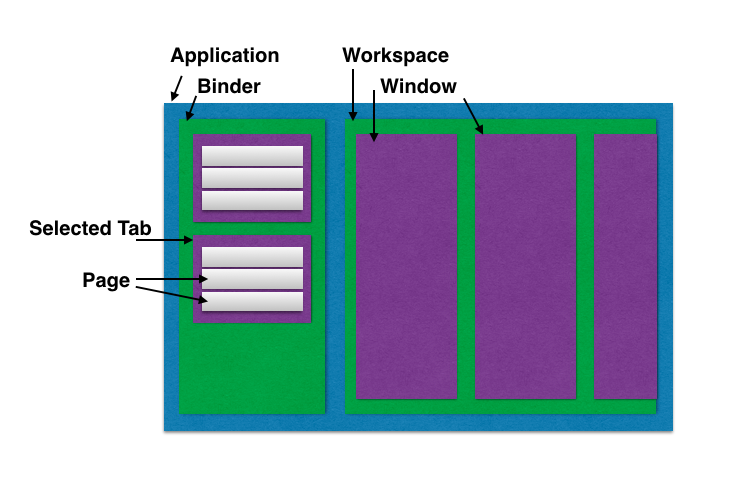
\includegraphics[width=0.8\textwidth]{Figures/WireframeDesign.png}
  \caption{Wire frame design, Shows the location of the functional elements of
  the design and their relative positions}
  \label{fig:wireframe}
\end{figure}


The left side of the application is dedicated to the navigation
interface with tabs and pages displayed with buttons to create new and
remove old.

The workspace is a container for the open pages in the application, each
page is a different component depending on what type the page is. For
example a search page renders a Search component and an index page
renders an Index component. This allows for easy addition of new window
types to the system as each is implemented in a separate file.

The initial design was implemented with the standard HTML entities ``li''
for list and ``button'' for actions. Later in the design process these
were replaced with components form a third party library of elements. The library
provides styled components that can be used in place of standard HTML. 
The styled components also follow the design specification called
``material design''.\footnote{\url{https://design.google.com/spec/} for more
information} This design specification defined rules for positioning, colouring
and other visual semantics that give the application a professional feel and 
also giving the design consistency with other applications that also use 
this style.

Changing the visual design of the system proved to be a simple task, this is
mostly due to the choice of technology. Browserify and React.js both contributed
by allowing a third party library\footnote{\url{http://www.material-ui.com/}} to 
be easily imported and replace the unstyled components.
